\chapter{Background}
In this chapter we will discuss main topics from Classical Mechanics and refresh out knowledge about common neural network architectures. This will be needed to understand the working of our Physics informed networks in chapter Methods.
 
\section{Classical Mechanics}
The classical physics are most important science to understand the laws which govern how mass object behaves in our reality. Such science is called the Classical Mechanics. It tend to describe how the mass moves in space. Simply the movement manifests through forces applied on the matter. Sir Isaac Newton for this observed phenomena gave a laws which masses should obey  \cite{ClassPhy}
\begin{itemize}
	\item Newton's 1st law: Unless acted on by an outside force the natural motion of an object is constant velocity
	\item Newton’s 2nd law: The effect of an applied force $\mathbf{F}$ upon an object of mass
	m is to induce an acceleration $\mathbf{a}$ such that $$\mathbf{F}=m\mathbf{a}$$
	If mass is constant we can introduce momentum $\mathbf{p}$.
	$$\mathbf{F}=\frac{d\mathbf{p}}{dt}$$ \\
	Derivation of the momentum in time t is a force. 
	With this equation we can obtain momentum as $$\mathbf{p}=m\mathbf{v}$$ where v is velocity.
	\item Newton’s 3rd law: If an object applies a force $\mathbf{F}$ on a second object, then the second object applies an equal and opposite force $-\mathbf{F}$ on the first object.\\
	In the physics it is most famous law and it is often referenced as  \textit{actio = reactio} from latin.
\end{itemize}
With application of  those laws we can describe the movement of some matter or body in space.
One of the easiest systems which obeys those laws is harmonic oscilator.
\subsection{Harmonic Oscilator}
Harmonic Oscilator is  system  in classical physics which describes the situation where body is displaced from equilibirium position and it experience the restoring force $\mathbf{F}$ proportional to its displacement.\cite{osci2} This system is described with Ordinary Differential Equation of second order : 
\begin{equation}
	m\ddot{\mathbf{x}}(t) = -k\mathbf{x}(t) \texttt{,   } \mathbf{x}(0)= \mathbf{x}_0
\end{equation}
We will consider this system as one dimensional $\mathbf{x}= x$
in which the harmonic motion is along straight line, the motion is said to be simple harmonic motion \cite{osci}. In the system $k$ is stifness of the spring and $m$ mass of the connected object.  To show the simple harmonic motion let us solve the equation.\\
First we will build the the linear system of equations to get the first order ordinary differential equation in form: \begin{equation}
	\ddot{\mathbf{z}}= \mathbf{A}\mathbf{z} + \mathbf{b}u.
\end{equation}
We are beginning with parameter $z$:
\begin{eqnarray}
	z_1 &=& x\\
	z_2 &=& \dot{x}\\
	\dot{z}_1 &=& \dot{x} = z_2\\
	\dot{z}_2 &=& \ddot{x} = -\frac{k}{m}z_1 
\end{eqnarray}
With this we got:
\begin{equation}
	\begin{bmatrix}
		\dot{z_1}\\
		\dot{z_2}\\
	\end{bmatrix} = \begin{bmatrix}
	0 & 1\\
	-\frac{k}{m} & 0\\
	\end{bmatrix}
	\begin{bmatrix}
		z_1\\
		z_2\\
	\end{bmatrix}
\end{equation}
We got differential ordinary equation which is homogeneous ($\mathbf{b}=0$). To solve this Problem we need to refresh the knowledge of solving the ODEs 

\subsection{Analytical solution of Ordinary Differential Equations}
A Differential Ordinary Equation of the first order is defined as:
\begin{equation}
\label{eq:diff}
\dot{\mathbf{z}}= \mathbf{A}\mathbf{z} + \mathbf{b}u \texttt{, }\mathbf{z}(0) = \mathbf{z}_0
\end{equation}
Before we show analytical solution of mentioned linear system, let us solve first the simplest case:
 
\begin{equation}
	\dot{z}(t)= az(t) + bu \texttt{, }z(0) = z_0
\end{equation}
Every solution of ODE has homogeneous $z_{hom}$ and particular solution $z_{par}$
\begin{equation}
	z(t) = z_{hom} + z_{par}.
\end{equation}
When we calculate de homogeneous solution we set $b=0$ and we precede with simple integration.
\begin{equation}
	\int\frac{dz}{z} = \int adt
\end{equation}
\begin{equation}
	\boxed{z_{hom}= c\exp(at)}
\end{equation}
To find particular solution we will create it with variation of the constants method.\\
We define:
\begin{equation}
	z_{part}= c(t)\exp(at)
\end{equation}
and we will put it in the differential equation
\begin{eqnarray}
	\dot{z}_{part}(t)&=& az_{part}(t) + bu(t),\\
	a\exp(at)c(t)+ \exp(at)\dot{c}(t)&=& a\exp(at)c(t) + bu(t),\\
	\dot{c}(t) &=& \exp(-at)bu(t).
\end{eqnarray}
After integration of $\dot{c}$ we get:
\begin{equation}
	\boxed{z_{part}= c(0)\exp(at) + \int^t_0 \exp(at-\tau)bu(\tau)d\tau}
\end{equation}
With inclusion of the Initial condition $z(0) = z_0$ we get final form of the solution \\
\begin{equation}
	\boxed{z= \underbrace{z_0\exp(at)}_\text{homogeneous} + \underbrace{\int^t_0 \exp(a(t-\tau))bu(\tau)d\tau}_\text{particular} }.
\end{equation}
Let so go back and solve the equation \ref{eq:diff}.\\
Obtaining the solution goes similar to simple case but it is vectorized.\\
The solution is made by homogeneous and particular solution as above.\\
\begin{equation}´
	\mathbf{z}=\mathbf{z}_{hom} + \mathbf{z}_{in}
\end{equation} 
Lets assume from the example what we have done previously that our homogeneous solution is defined as:
\begin{equation}
	\mathbf{z}_{hom}=\exp(\mathbf{A}t)\mathbf{c}
\end{equation}
This is easy to prove trough Taylor series of the $\exp(\mathbf{A}t)$.
\begin{equation}
	\exp(\mathbf{A}t) = \sum^{\infty}_{i=0}\frac{(\mathbf{A}t)î}{i!} = \mathbf{I}+ \mathbf{A}t+\mathbf{A}^2 \frac{t^2}{2!}+ \mathbf{A}^3 \frac{t^3}{3!} + \mathcal{O}(t^4)
\end{equation}
\begin{eqnarray}
	\frac{d\exp(\mathbf{A}t)}{dt} &=& \mathbf{A}+\mathbf{A}^2 t+ \mathbf{A}^3 \frac{t^2}{3!} + \mathcal{O}(t^3)=\\
	&&\mathbf{A}\left(\mathbf{I}+ \mathbf{A}t+\mathbf{A}^2 \frac{t^2}{2!}\right) + \mathcal{O}(t^3)\\
	&&\mathbf{A}\exp(\mathbf{A}t)
\end{eqnarray}
Lets put it in the equation
\begin{eqnarray}
	\dot{\mathbf{z}}_{hom}&=& \frac{d\exp(\mathbf{A}t)}{dt}\mathbf{c} =\\
	&&\mathbf{A}\exp(\mathbf{A}t)\mathbf{c} =\\
	&& \mathbf{A}\mathbf{z}_{hom}
\end{eqnarray}
and the homogeneous solution
\begin{equation}
	\boxed{
	\mathbf{z}_{hom} = \exp(\mathbf{A}t)\mathbf{c}}
\end{equation}
fulfills the equation.\\
With the variation of the constant method we obtain the particular solution:
\begin{equation}
\exp(\mathbf{A}t)\mathbf{c}(0)+ \int^t_0 \exp(\mathbf{A}(t-\tau))\mathbf{b}u(\tau)d\tau
\end{equation}
With inclusion of the initial condition $z(0) = z_0$ we get final form of the solution \\
\begin{equation}
	\boxed{\mathbf{z}= \underbrace{\exp(\mathbf{A}t)\mathbf{x}_0}_\text{homogeneous} + \underbrace{\int^t_0 \exp(\mathbf{A}(t-\tau))bu(\tau)d\tau}_\text{particular}}.
\end{equation}\\
In our work the most important part is homogeneous solution and to obtain that we should use standard practice to solving it.\\
\begin{itemize}
	\item Find eigenvalues and eigenvectors- Every matrix with full rank is diagonalizable 
	\begin{eqnarray}
		\mathbf{A} &=& \mathbf{V}\mathbf{D}\mathbf{V}^{-1}\\
		\mathbf{D} &=& \texttt{diag}(\{\lambda_1,...,\lambda_i,...\lambda_n\}) \text{    Eigenvalues}\\`
		\mathbf{V} &=& \left[\mathbf{v}_1|...|\mathbf{v}_i|...|\mathbf{v}_n\right] \text{    Eigenvectors}
	\end{eqnarray}
	It is easily obtained through characteristic polynomial $p(\lambda) =\det(\mathbf{A}-\mathbf{I}\lambda)=0$
	
	\item To find general solution we need to transform the $\dot{\mathbf{z}}= \mathbf{A}\mathbf{z}$
	\begin{eqnarray}
		\dot{\mathbf{z}} &=& \mathbf{V}\mathbf{D}\mathbf{V}^{-1}\mathbf{z}\\
		\underbrace{\mathbf{V}^{-1}\dot{\mathbf{z}}}_\text{} &=& \mathbf{D}\underbrace{\mathbf{V}^{-1}{\mathbf{z}}}_\text{}\\
		\dot{\boldsymbol{\Theta}}&=&\mathbf{D}\boldsymbol{\Theta}
	\end{eqnarray}
	This system is now trivial to solve.
	\item Set it in general solution $\Theta_i=c_i\exp(\lambda_i t)$ 
	In case of repeated eigenvalue we should use $\Theta_i=c_i \frac{t^r}{r!} \exp(\lambda_i t)$ where $r$ is number of repetitions.
	It will came up from the eigenvectors. 
	\item back-substitute $\mathbf{z}$
	\begin{eqnarray}
		\mathbf{z} &=& \mathbf{V}\boldsymbol{\Theta} =\sum^n_{i=1}\mathbf{v}_i\Theta_i\\
		\mathbf{z} &=& \sum^n_{i=1} \mathbf{v}_i\underbrace{c_i\exp(\lambda_i t)}_\text{\Theta}
	\end{eqnarray}
	\item apply initial conditions
	\begin{eqnarray}
	\mathbf{z}(0) = \sum^n_{i=1} \mathbf{v}_i c_i = \mathbf{V}\mathbf{c} &=&\mathbf{z}_0\\
	\mathbf{c} &=&\mathbf{V}^{-1}\mathbf{z}_0
    \end{eqnarray}
	
\end{itemize}

In this procedure we obtained the homogeneous solution. The particular solution is in some cases trivial but in some not solvable analytically due to $\mathbf{b}u(t)$. It is possible that it is nonlinear function. 
In those cases we use numerical methods to obtain the solutions.

\subsection{Numerical solution of Ordinary Differential Equations}
For every every ODE there is solution, sometimes there is no analytical solution but we can obtain numerical one trough numerical integrators. 
Still numerical solutions are only approximations of the analytical solution. Due to their stability we differ two categories of one-step methods and that are explicit and implicit methods.\\
\begin{itemize}
	\item explicit methods are trivial to calculate because the next step is dependent only on the previous step:
	\begin{equation}
		x(t_{i+1}) = x(t_i) + h\Phi(x(t_i)),t_i)
	\end{equation}
	\item implicit methods are chalenging because the next step is dependent on itself.
	\begin{equation}
		x(t_{i+1}) = x(t_i) + h\Phi(x(t_{i+1})),t_{i+1})
	\end{equation}
To obtain the step it is needed to know  function $\Phi$ and solving a next step trough some method like  for example Einstein-Raphson method. 
\end{itemize}
To assure the stability and correctness of the methods we need to set some properties.
The properties that the every one-step method should have, are Consistency and Convergence.\\

The Consistency are proven over local discretisation error.
Let say that for $(x,y)\in  \mu = \mu(\eta)$ is a solution for the ODE $\mu^{'} = f(\eta,\mu), \mu(x)=y$,then the discretisation error is
\begin{equation}
	le(x,y;h) = \mu(x+h)-\mu{x}-h\Phi(x,y;h)
\end{equation}
and discretisation error per step
\begin{equation}
	\Delta(x,y;h)=\frac{le(x,y;h)}{h}. 
\end{equation}
A one-step method is consistent if
\begin{equation}
	\lim_{h\rightarrow 0} \Delta(x,y;h) = 0.
\end{equation}
For the method to be convergent need to be consistent. The general definition of convergency is
\begin{equation}
\lim_{h\rightarrow 0} \Phi(x,y;h) = f(x,y)
\end{equation}
To prove this we should look for the consistency and convergency rank.
\begin{itemize}
	\item Consistency rank $p$\begin{equation}
		||\Delta(x,y;h)||\leq Kh^p
	\end{equation}
\item Convergency rank $p$
\begin{eqnarray}
	E(h) &=& \max_{j=0,1,...N}||y_j-y(x_j)||\text{ global discretisation error }\\
	\lim_{h\rightarrow 0}E(h) &=& 0 \text{ Convergence}\\
	E(h) &\leq&  Kh^p
\end{eqnarray}



\end{itemize} 
This properties are highly important to know because we will use for the experiments mostly the Runga-Kutta methods which are based on those properties.\\
Most important for us are
\begin{itemize}
	\item Euler method
		\begin{equation}
			x_{i+1} = x_i + hf(x_i,t_i)
		\end{equation}
	\item Runge-Kutta 4 Method(RK4)
		\begin{eqnarray}
			K_1 &=& f(x_i,t_i)\\
			K_2 &=& f(x_i + \frac{h}{2}K_1,t_i +\frac{h}{2})\\
			K_3 &=& f(x_i + \frac{h}{2}K_2,t_i+\frac{h}{2})\\
			K_4 &=& f(x_i + hK_3,t_i +h)\\
			x_{i+1} &=& x_i + \frac{h}{6}(K_1 + 2K_2 +2K_3 +K_4)
		\end{eqnarray}	
	\item Dormand- Prince method is most accurate method for obtaining he solutions of ODEs\cite{dopri5}.
	It is widely used in experiments.\\
		
\end{itemize}
\subsection{Solving the harmonic oscilator}
In one of the previous subsections we obtained the first order ODE for harmonic oscilator and we described how it should be solved.
\begin{equation}
	\begin{bmatrix}
		\dot{z_1}\\
		\dot{z_2}\\
	\end{bmatrix} = \begin{bmatrix}
		0 & 1\\
		-\frac{k}{m} & 0\\
	\end{bmatrix}
	\begin{bmatrix}
		z_1\\
		z_2\\
	\end{bmatrix}\text{   , }\mathbf{z}_0 = \begin{bmatrix}
x_0\\
v_0\\
\end{bmatrix}
\end{equation}
Through the system Matrix $A = \begin{bmatrix}
	0 & 1\\
	-\frac{k}{m} & 0\\
\end{bmatrix}$ we got complex eigenvalues, which are $\lambda_1 = i\sqrt{\frac{k}{m}}$ and $\lambda_2 = -i\sqrt{\frac{k}{m}}$.\\
General solution of this problem is
\begin{equation}
	z_1 = x = c_1\exp(i\sqrt{\frac{k}{m}}t) + c_2\exp(i\sqrt{-\frac{k}{m}}t)
\end{equation}
With applying of the euler formula:
\begin{equation}
	\exp(iat)=\cos(at) + i\sin(at)
\end{equation}
We get simplified solution
\begin{eqnarray}
	z_1 &= x =& (c_1+c_2)\cos\left(\sqrt{\frac{k}{m}}t\right) + (c_1-c_2)i\sin\left(\sqrt{\frac{k}{m}}t\right)\\
	z_2 &= \dot{x} =& -(c_1+c_2)\sqrt{\frac{k}{m}}\sin\left(\sqrt{\frac{k}{m}}t\right)+(c_1-c_2)\sqrt{\frac{k}{m}}i\cos\left(\sqrt{\frac{k}{m}}t\right).
\end{eqnarray}
Now we can apply initial conditions
\begin{eqnarray}
x(0)=x_0 = c_1 + c_2,\\
\dot{x}(0)=v_0 = i(c_1-c_2).
\end{eqnarray}
The velocity in our cases is an real number which we can assume that constants $c_1$ and $c_2$ are equal. 
This simplifies our equations  and we can substitute $x_0 = c_1 +c_2$
\begin{eqnarray}
	z_1 &= x =& x_0\cos\left(\sqrt{\frac{k}{m}}t\right),\\
	z_2 &= \dot{x} =& -x_0\sqrt{\frac{k}{m}}\sin\left(\sqrt{\frac{k}{m}}t\right)
\end{eqnarray}
The is harmonic at we can se that clearly because it is periodic and we can read an angle velocity of periodic movement $\omega = \sqrt{\frac{k}{m}}$,
\begin{eqnarray}
	z_1 &= x =& x_0\cos\left(\omega t\right)\\
	z_2 &= \dot{x} =& -x_0\omega\sin\left(\omega t\right)
\end{eqnarray}
\subsection{Langrange and Hamiltonian Equations}
In robotics, research and model creation of the robot models are not only one-bodied system. Mostly they are are rigid-body systems like a manipulator which has N degrees of freedom. Every of the joints and links have own properties like mass, friction, etc.\\
The Kinematic of the model and irreversibility is possible to calculate with mathematic methods. Kinematic is just establishing the function which with correct input like angles of joints $q$ give as an output in form of target position of the endeffector. This easy easy to establish with Denavit–Hartenberg convention.  On the other hand determining Dynamics is not trivial task. The Dynamic creates trajectory which is in form of ODE.\\
There is one most popular method to solve and establish Dynamics of the model and that are Lagrange Equations.
\subsubsection{Lagrange Equations}
Langrage Equations are derived from D’Alambert Principle which is an alternative to the Newton's second law\cite{ClassPhy}:
\begin{equation}
	\mathbf{F} = m\mathbf{a}
\end{equation}   
In the case of the rigid body:
\begin{equation}
	\mathbf{F}_i = \sum_i{m_i \mathbf{a}_i}
\end{equation}
To derive Lagrangian Equations which describes dynamics we need first to define constraints. Let us define homonomic constraints.
For $N$ bodies B = $\{\mathbf{r}_1,...,\mathbf{r}_i,...,\mathbf{r}_N\}\text{ ; } \mathbf{r}_i=\mathbf{r}_i(q_1,...,q_i,...,q_n, t)$
\begin{equation}
	\boxed{G_k(\mathbf{r}_1,..,\mathbf{r}_i,..,\mathbf{r}_n,t)=0\text{ for}k=1,..M}
\end{equation}
Where the $q_i$ are generalized coordinates and the
parameters are also constrained as $3\cdot M\cdot N = n$.\\
In case of two dimensional N-Pendulum some of that constraints would look like:
\begin{equation}
	G_i := \left|\left|\mathbf{r}_i - \mathbf{r}_{i+1}\right|\right| - d_i = 0
\end{equation}
This says that the distance between two neighboring joints are constant.
holonomic constraint defines the relation between bodies $\r_i$ on some configuration space $\mathcal{A}$.
Lets go back to the second newton law and lets apply holonomic constraint. With holonomic constraint we can spilt $\mathbf{F}$ on constraint force $\mathbf{F}^c$ and apllied force $\mathbf{F}^a$.
\begin{equation}
	\mathbf{F} =\mathbf{F}^c + \mathbf{F}^a
\end{equation}
Now we will apply virutal Work principle, which comes from orthogonality of virtual displacement and constraint forces \cite{ortho}
\begin{equation}
	\boxed{\sum_i{\mathbf{F}_i^c \cdot \underbrace{\delta \mathbf{r}_i}=0}_\text{virtual displacement}}
\end{equation}
to the constrained Newton's second law we get following formula which is D'Alambert principle\cite{dalam}:
\begin{eqnarray}
	 \mathbf{F}^c_i &=& \mathbf{F}_i- \mathbf{F}^a_i\\
	 \sum_i{\mathbf{F}_i^c \cdot \delta \mathbf{r}_i} &=& \sum_i{(\mathbf{F}_i- \mathbf{F}^a_i) \cdot \delta \mathbf{r}_i}\\
	 \sum_i{(\mathbf{F}_i- m_i\ddot{\mathbf{r}}_i) \cdot \delta \mathbf{r}_i}&=&0\text{    D'Alambert Principle}
\end{eqnarray}\\
If we need virtual displacement for the generalized coordinates:
\begin{equation}
	\delta\mathbf{r}_i = \sum_j^n{\frac{\partial\mathbf{r}_i}{\partial q_j}\cdot \delta q_j}
\end{equation}
Now we can derive Langrange Equations applying last equation to D'Alambert principle:
\begin{eqnarray*}
\sum_i^N{\mathbf{F}_i \cdot \delta \mathbf{r}_i} &=& \\ \sum_i^N{\mathbf{F}_i\sum_j^n{\frac{\partial\mathbf{r}_i}{\partial q_j}\cdot \delta q_j}}&=&\\
\sum_j^n{\delta q_j\underbrace{\sum_i^N{\mathbf{F}_i}\frac{\partial\mathbf{r}_i}{\partial q_j}}_\text{$Q_j$}}&=&\boxed{\sum_j^n{\delta q_j\cdot Q_j}}\\
\sum_i^N{m_i\ddot{\mathbf{r}}_i \cdot \delta \mathbf{r}_i}&=&\\
\sum_i^N{m_i\ddot{\mathbf{r}}_i \sum_j^n{\frac{\partial\mathbf{r}_i}{\partial q_j}\cdot \delta q_j}}&=&
\sum_j^n{\delta q_j\sum_i^N{m_i\ddot{\mathbf{r}}_i\frac{\partial\mathbf{r}_i}{\partial q_j}}}\\
\text{with substitution of: } \frac{\partial\dot{\mathbf{r}_i}}{\partial \dot{q_j}} &=& \frac{\partial}{\partial \dot{q_j}}\left(\frac{d\mathbf{r}_i}{dt} + \sum^N_i{\frac{\partial \mathbf{r_i}}{q_j}\dot{q_j}}\right) = \frac{\partial \mathbf{r_i}}{q_j}\\
\sum_i^N{m_i\ddot{\mathbf{r}}_i \sum_j^n{\frac{\partial\mathbf{r}_i}{\partial q_j}\cdot \delta q_j}}&=&
\sum_j^n{\delta q_j\sum_i^N{m_i\ddot{\mathbf{r}}_i\frac{\partial\dot{\mathbf{r}_i}}{\partial \dot{q_j}}}}\\
\text{with: }\sum_i^N{\frac{d}{dt}m_i\dot{\mathbf{r}}_i\frac{\partial\dot{\mathbf{r}_i}}{\partial \dot{q_j}}} &=& \sum_i^N{m_i\ddot{\mathbf{r}}_i\frac{\partial\dot{\mathbf{r}_i}}{\partial \dot{q_j}}+m_i\dot{\mathbf{r}_i}\frac{d}{dt}\frac{\partial \mathbf{r}_i}{\partial q_j}}\\
\sum_j^n{\delta q_j\sum_i^N{m_i\ddot{\mathbf{r}}_i\frac{\partial\mathbf{r}_i}{\partial \dot{q_j}}}} &=& \sum_j^n{\delta q_j\sum_i^N{\frac{d}{dt}\left(m_i\dot{\mathbf{r}_i}\frac{\partial\dot{\mathbf{r}_i}}{\partial \dot{q}}\right)-m_i\dot{\mathbf{r}_i}\frac{\partial\dot{\mathbf{r}_i}}{\partial q}}}\\
\end{eqnarray*}
We get this equation
\begin{equation}
\boxed{\sum_i^N{m_i\ddot{\mathbf{r}}_i \cdot \delta \mathbf{r}_i} =\sum_j^n{\delta q_j\left[\frac{d}{dt}\frac{\partial}{\partial \dot{q_j}}\left(\sum_i^N\frac{1}{2}m_i\dot{\mathbf{r}_i}^2\right)-\frac{\partial}{\partial \dot{q_j}}\left(\sum_i^N\frac{1}{2}m_i\dot{\mathbf{r}_i}^2\right)\right]}}
\end{equation}
With those two made equations we can finally put it togehter in D'Alambert Principle formula:
\begin{equation}
	\sum_j^n{\delta q_j\left[\frac{d}{dt}\frac{\partial}{\partial \dot{q_j}}\left(\sum_i^N\frac{1}{2}m_i\dot{\mathbf{r}_i}^2\right)-\frac{\partial}{\partial q_j}\left(\sum_i^N\frac{1}{2}m_i\dot{\mathbf{r}_i}^2\right)- Q_j\right]} =0 
\end{equation}
This Equation is almost complete, we need to define the energies and their specifications

\begin{itemize}
	\item Kinetic Energy - Energy possessed by bodies due to their motion.\\
	The Formula for kinetic energy is
	\begin{equation}
		T(q,\dot{q}) = \sum_i^N\frac{1}{2}m_i\dot{\mathbf{r}_i}^2
	\end{equation}
	\item Potential Energy - Energy held by body becuase of its relative position to other bodies or other target.\\
	There is many types of potential energy:\\
	Pendelum - $U(q=h)=mgh$\\
	Oscilator - $U(q)=\frac{kq}{2}$ 
\end{itemize}
In the Formula $\mathbf{Q}$ is generalized force and it is created from the gradient of the potential energy and it is conservative :
\begin{equation}
	\mathbf{Q_j} =- \sum^N_i \nabla_{\mathbf{r_i}}U(q)\frac{\partial\mathbf{r_i}}{\partial q_j}= -\frac{\partial U}{\partial q_j}
\end{equation} 
Potential Energy is only dependent on position of the bodies $\frac{\partial U}{\partial \dot{q}} = 0$.\\
The Lagrange Equations for holonomic constrains and conservative force is defined as:
\begin{eqnarray}
\frac{d}{dt}\frac{\partial}{\partial \dot{q_j}}\left(T-U\right)-\frac{\partial}{\partial q_j}\left(T-U\right) =0\\
\frac{d}{dt}\frac{\partial}{\partial \dot{q_j}}\mathcal{L}-\frac{\partial}{\partial q_j}\mathcal{L} =0
\end{eqnarray}
$\mathcal{L}$ is called Lagrangian.
\subsubsection{Hamiltonian Equations}
To derive Hamiltonian Equations we need an Lagrangian $\mathcal{L}$.
We have two famous derivation of Langrangian and that are:
\begin{equation}
	\frac{\partial\mathcal{L}}{\partial \mathbf{q}} = \dot{\mathbf{p}}
\end{equation}
\begin{equation}
	\frac{\partial\mathcal{L}}{\partial \dot{\mathbf{q}}} = \mathbf{p}
\end{equation}
Through Legendre Transformation we can obtain Hamiltonian $\mathcal{H}$
\begin{equation}
	\mathcal{H}(\mathbf{q},\dot{\mathbf{q}},\mathbf{p},t) = \sum_i^N  \dot{\mathbf{q}_i} \cdot \mathbf{p}_i -\mathcal{L}(\mathbf{q},\dot{\mathbf{q}},t)
\end{equation}
With total derivation\cite{ham} we get
\begin{eqnarray}
	d\mathcal{H} &=& \sum_i^N\left[ \dot{\mathbf{q}} d\mathbf{p}_i +  \mathbf{p}_i d\dot{\mathbf{q}_i} - \frac{\partial\mathcal{L}}{\partial \mathbf{q}_i} d\mathbf{q}_i - \frac{\partial\mathcal{L}}{\partial \dot{\mathbf{q}_i}} d\dot{\mathbf{q}_i}\right] - \frac{\partial\mathcal{L}}{\partial t} dt\\ 
	&=& \sum_i^N\left[ \dot{\mathbf{q}} d\mathbf{p}_i +  \mathbf{p}_i d\dot{\mathbf{q}_i} - \dot{\mathbf{p}_i} d\mathbf{q}_i - \mathbf{p}_i d\dot{\mathbf{q}_i}\right] - \frac{\partial\mathcal{L}}{\partial t} dt\\
	&=&\sum_i^N\left[ \dot{\mathbf{q}} d\mathbf{p}_i  - \dot{\mathbf{p}_i} d\mathbf{q}_i\right] - \frac{\partial\mathcal{L}}{\partial t} dt\\
\end{eqnarray}
On the other hand we want hamiltonian which is dependent on canoical moment and generalized coordinates $\mathcal{H}=\mathcal{H}(\mathbf{q},\mathbf{p},t)$
In that case the total derivation of Hamiltonian $\mathcal{H}$ is
\begin{equation}
	d\mathcal{H} = \sum_i^N\left[\frac{\partial \mathcal{H}}{\partial \mathbf{q}_i}d\mathbf{q}_i + \frac{\partial \mathcal{H}}{\partial \mathbf{p}_i}d\mathbf{p}_i\right] + \frac{\partial\mathcal{H}}{\partial t} dt
\end{equation}
With comparing both equivalent derivations we can define the equations of motion:
\begin{equation}
	\dot{\mathbf{p}} = -\frac{\partial \mathcal{H}}{\partial \mathbf{q}}
\end{equation}
\begin{equation}
	\dot{\mathbf{q}} = \frac{\partial \mathcal{H}}{\partial \mathbf{p}}
\end{equation}
\begin{equation}
	\frac{\partial\mathcal{H}}{\partial t} = - \frac{\partial\mathcal{L}}{\partial t}
\end{equation}
Hamiltonian equations are very useful because in the case $\frac{\partial\mathcal{H}}{\partial t} = 0$ our Total Energy $\mathcal{H} = E = T + U$ is conserved and often we can derive time independent motion. BLU
\section{Neural Network Architectures}
At the beginning of our research we experimented with feedforward networks and recurrent networks.  
\subsection{Deep forward Network - Multilayer Perceptron }
Feedforward networks like Multilayer perceptron approximates a certain function $\mathbf{f(\mathbf{x})}$. As MLP function we will show it as a mapping $\mathbf{f}(\mathbf{x}|\Theta)$.\\
The main goal of feedforward network is to fit the model so that the we get best approximation. Fit the model means to learn the parameters of the model trough optimizing procedure.\\
Multiplayer perceptron is fully connected feedforward neural network. The nodes of the MLP are often called neurons and they build a layer. A minimal MLP has three consecutive layers: which form complete bipartite graph.\\
Mathematical expression of one neuron:
\begin{equation}
	y = \sigma(\sum_i{w_i \cdot x_i} + b) 
\end{equation}
Mathematical expression of the feedforward layer network:
\begin{equation}
	\mathbf{h}^{(k+1)} =\sigma\left(\mathbf{W}^{(k)}\mathbf{h}^{(k)} + \mathbf{b}^{(k)}\right)
\end{equation} and we can see graphical representation in \ref{mlp}
In this equation $\sigma$ is called activation function, 
$\mathbf{W}$ as weights and $\mathbf{b}$ as bias which are our parameters $\Theta =\{\mathbf{W},\mathbf{b}\}$.\\
\begin{figure}[h!]
	\centering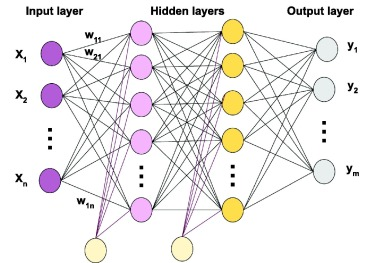
\includegraphics[width=8cm]{chapters/chapter2/mlp}
	\caption{Multilayer perceptron\cite{mlppic}}
	\label{mlp}
\end{figure}
The activation function in the network introduces non linearity to improve approximation capability.\\




\subsection{Recurrent Neural Networks}
Reccurent Neural Networks are very interesting concept of Neural Network architecture. It is mostly used for speech recognition but for a time series\cite{mlprnn}.\\
Architecture of this Neural Network depends on which data we work.
There is three types which we can use\cite{rnntypes}:
\begin{itemize}
	\item many to many\\
	This type is used for speech recognition we use a dataset which has sentences and it outputs some values which could be understood from other model. Fo example translation or video captioning
	\item one to many\\
	used for the time series data from one input we can create recurrence that represent a time point with new output. From one input we get more outputs. time-series can be for example music generation.
	\item many to one\\
	from many outputs we get only one output. This is very good model for example spam detection
\end{itemize}
Let say that we have a sequence $S = \{\mathbf{x}^0,\mathbf{x}^1,...,\mathbf{x}î,..\mathbf{x}^n\}$. the first element $\mathbf{h}^0$ will be initialized as 0.
The architecture of the RNN-cell\cite{rnn} described in mathematical formulation 
\begin{eqnarray*}
	\mathbf{h}^{(i)} &=& \sigma(\mathbf{W}_{hh} \cdot \mathbf{h}^{(i-1)} + \mathbf{W}_{hx}\mathbf{x}^{(i-1)} + \mathbf{b}_h)\\
	\mathbf{y}^{(i)} &=& \sigma(W_{yh}\cdot \mathbf{h}^{(i)} + \mathbf{b}_y)
\end{eqnarray*} and graphical appearance is shown in \ref{rnn}
\begin{figure}[h!]
	\centering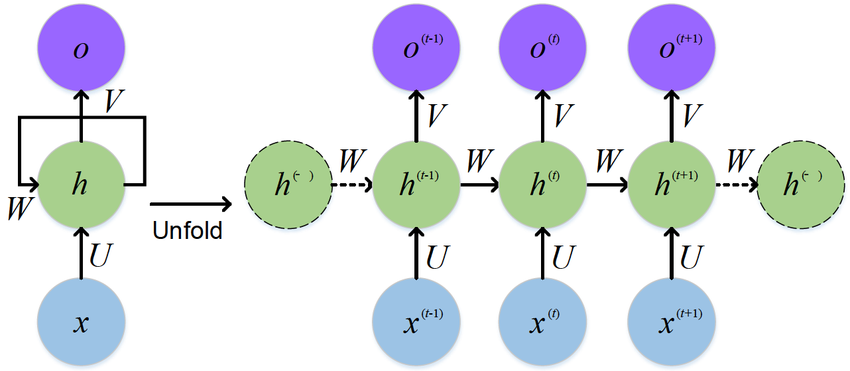
\includegraphics[width=8cm]{chapters/chapter2/rnn}
	\caption{Recurrent neural unit(many to many)\cite{rnn_picture}}
	\label{rnn}
\end{figure}

There is similar and better model then RNN and that is Gated Recurrent Unit called GRU.
We use it in same way as RNN but it his own unique architecture\cite{gru}:
\begin{eqnarray}
	r_t &=& \sigma(W_{ir} x_t + b_{ir} + W_{hr} h_{(t-1)} + b_{hr}) \\
	z_t &=& \sigma(W_{iz} x_t + b_{iz} + W_{hz} h_{(t-1)} + b_{hz}) \\
	n_t &=& \tanh(W_{in} x_t + b_{in} + r_t \odot (W_{hn} h_{(t-1)}+ b_{hn})) \\
	h_t &=& (1 - z_t) \odot n_t + z_t \odot h_{(t-1)}
\end{eqnarray} and we can see it in plot \ref{gru}
\begin{figure}[h!]
	\centering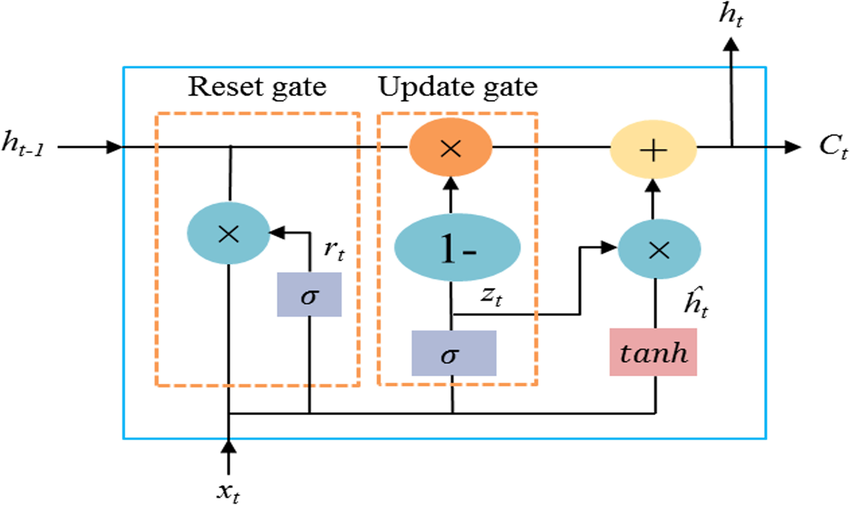
\includegraphics[width=8cm]{chapters/chapter2/gru}
	\caption{Gated recurrent unit\cite{gru_picture}}
	\label{gnn}
\end{figure}
The GRU unit is specific because it has reset gate $r_i$ and update gate $u_i$. Such architecture give better performance then at simple RNN.

\subsection{Activation functions and Loss functions}
In every neural architecture there is a activation function.
Most used activation functions are:
\begin{itemize}
	\item ReLU\\
	\begin{equation}
		\text{ReLU}(x) = max(x,0)
	\end{equation}
	This function passes only positive values.\\
	\begin{figure}[h!]
		\centering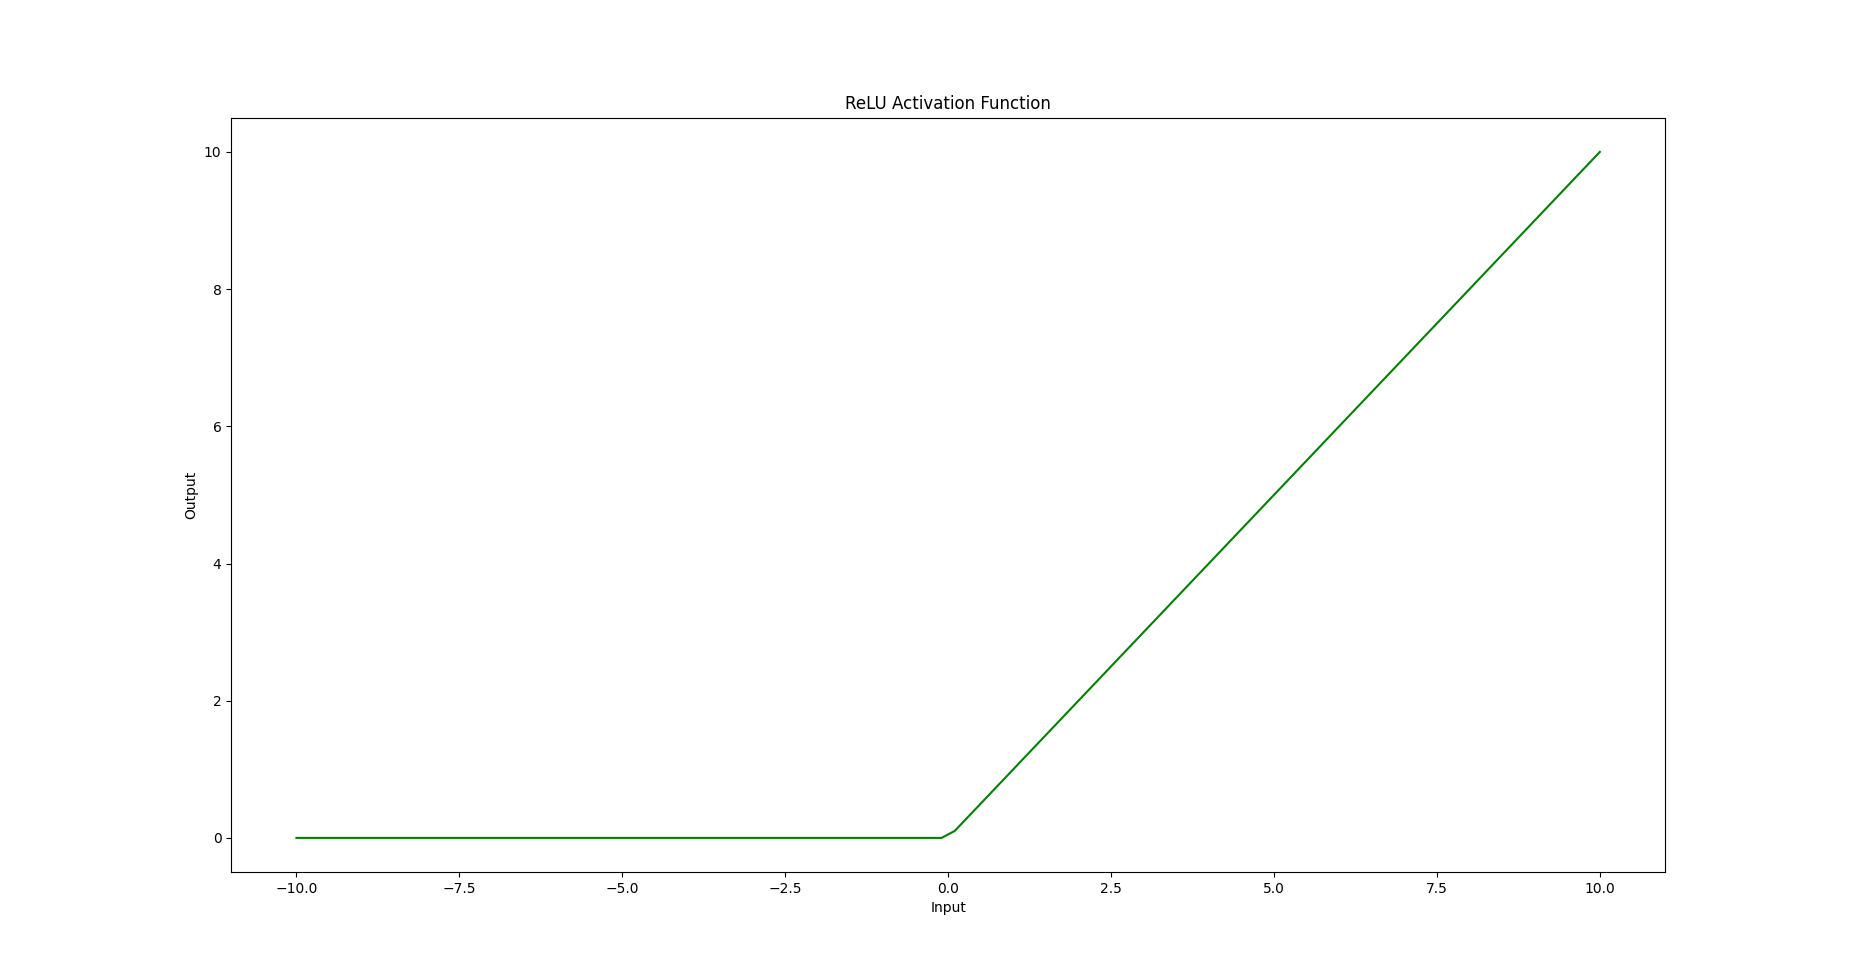
\includegraphics[width=8cm]{chapters/chapter2/relu}
		\caption{ReLU activation}
		\label{relu}
	\end{figure}
	\item tanH - It gives an output $y \in [-1,1]$\\
	\begin{figure}[h!]
		\centering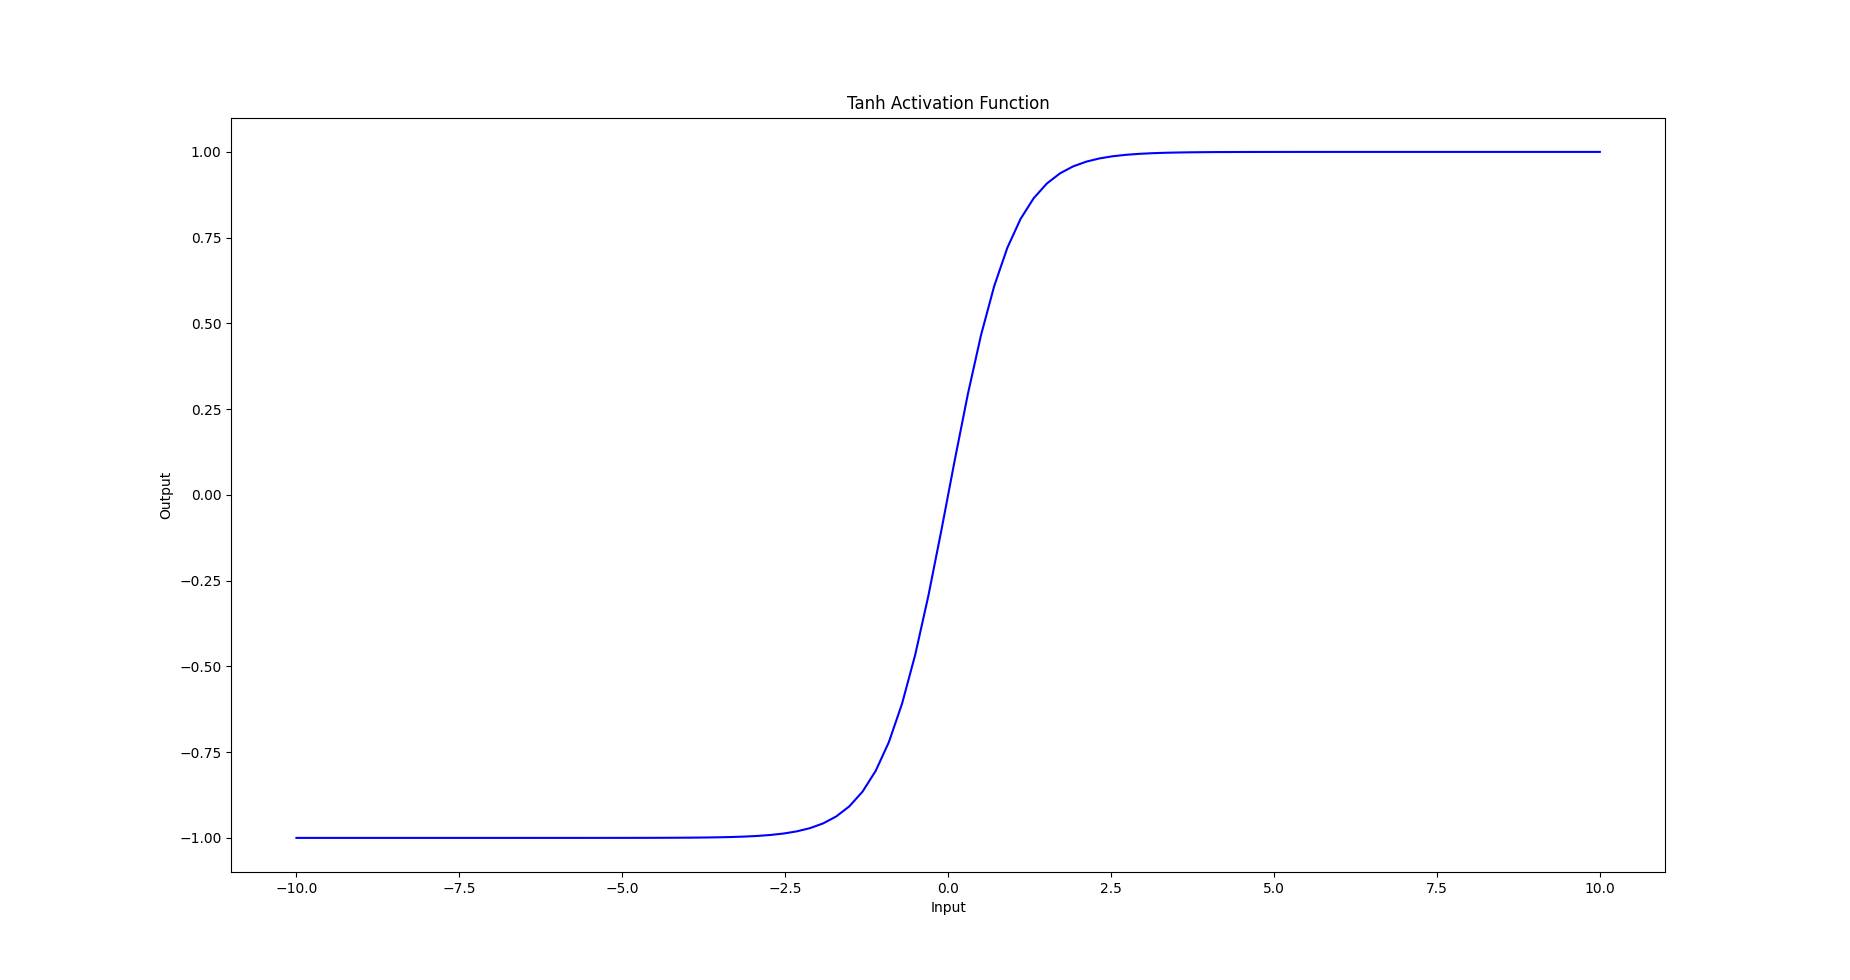
\includegraphics[width=8cm]{chapters/chapter2/tanh}
		\caption{Tanh activation}
		\label{tanh}
	\end{figure}
\end{itemize} 

Output layer has no activation function. it is connected to the loss function. The most used loss functions are:
\begin{itemize}
	\item Mean Absolute Error(MAE)
	\begin{equation}
		\text{MAE}(y,\hat{y}) = \frac{1}{N}\sum^N_i \left|y_i-\hat{y}_i\right|
	\end{equation}
	
	\item Mean Squared Error(MSE)
	\begin{equation}
		\text{MSE}(y,\hat{y}) = \frac{1}{N}\sum^N_i \left(y_i-\hat{y}_i\right)^2
	\end{equation}
	
	\item HuberLoss
	\begin{equation}
		\text{HuberLoss}(y,\hat{y};\delta) = \left\{\begin{matrix}
			\frac{1}{2}(y - \hat{y})^{2} & if \left | (y - \hat{y})  \right | < \delta\\
			\delta ((y - \hat{y}) - \frac1 2 \delta) & otherwise
		\end{matrix}\right.
	\end{equation}
	
\end{itemize}.

\subsection{Optimizers}
To do backpropagation we need an optimizer to update our learnable parameters. The easiest optimizer is stochastic gradient descent.
\begin{equation}
	\mathbf{W}^{(i+1)} =\mathbf{W}^{(i)}-\mu \frac{\partial Loss(z)}{\partial \mathbf{W}^{(i)}}
\end{equation}
There are more better one and for our use case we will use AdamW\cite{adamW}.

\subsection{Backpropagation of Neural Models}
After forward pass and calculated loss, we need to do just next steps Backward pass and optimization step.\\In backward pass we are computing the gradients of our learnable parameters to use it for the optimization of the model.\\
For example we will use stochstic gradient descent(SGD)
\begin{eqnarray}
	\mathbf{W}_{i+1} = \mathbf{W}_i - \gamma\cdot \frac{\partial Loss(z)}{\partial \mathbf{W}_i }\\
	\mathbf{b}_{i+1} = \mathbf{b}_i - \gamma\cdot \frac{\partial Loss(z)}{\partial \mathbf{b}_i }
\end{eqnarray} where $\gamma$ is a learning rate and one layered MLP
without bias $\mathbf{b}$.
\begin{eqnarray}
	\mathbf{z}_1 = \mathbf{W_0}\mathbf{y_0}\\ 
	\mathbf{y}_1 = \sigma(\mathbf{z}_1)\\
	\text{Loss}(y_1,\hat{y}) = \text{MSE}(y_1,\hat{y})
\end{eqnarray}
The obtaining the gradients of the weights is called backpropagation because for its calculation we need to apply chain rule for derivation.
\begin{equation}
\frac{\partial Loss(z)}{\partial \mathbf{W}_0}= \frac{\partial Loss(z)}{\partial \mathbf{y}_1} \cdot\frac{\partial \mathbf{y}_1}{\partial \mathbf{z}_1}\cdot	\frac{\partial \mathbf{z}_1}{\partial \mathbf{W}_0}
\end{equation}
Recurrent neural networks often fall as a victim of gradient vanishing or gradient exploding. In this manner the models doesn’t learn because the derivations calculated through backpropogation are to small or to big. It is important that gradients slowly decrease trough learning that whole model can generalize the data.
